\documentclass{standalone}
%
\usepackage{tikz}
\usetikzlibrary{backgrounds}
\usetikzlibrary{calc}
\usetikzlibrary{decorations.pathmorphing}
\usetikzlibrary{bending,arrows.meta}
\usepackage{xcolor}
%
\definecolor{space}{HTML}{0A2543}
\definecolor{earth}{HTML}{0089FA}
\definecolor{mars}{HTML}{DC7B4E}
\definecolor{mercury}{HTML}{846549}
\definecolor{glasses}{HTML}{08663D}
\definecolor{dida}{HTML}{FFDE00}
\definecolor{title}{HTML}{FBA706}
\definecolor{moon}{HTML}{AFAFAF}
\definecolor{craterm}{HTML}{616060}
\definecolor{linem}{HTML}{DBDBDB}
\definecolor{core1}{HTML}{FF5E16}
\definecolor{core2}{HTML}{FF9616}
\definecolor{core3}{HTML}{FFD016}
%
\usepackage{fontspec}
\setmainfont{Open Dyslexic}
%
\title{Fatti mercuriali}
\begin{document}
	\tikzset{partial ellipse/.style args = {#1:#2:#3}{insert path={+ (#1:#3) arc (#1:#2:#3)}}}
	\begin{tikzpicture}[background rectangle/.style={fill=white},show background rectangle,>={[inset=0,angle'=27]Stealth}]
		%title
		\draw [black,ultra thick,fill=title] (0,8) rectangle (30,11.5);
		\node at (14,9.8) {\textcolor{black}{\fontsize{90}{91}\selectfont Fatti mercuriali}};
		%mercury
		\begin{scope}[scale=2.5]
			\coordinate (E) at (2.6,0.4);
			\coordinate (F) at (3.7,0.7);
			\draw[fill=mercury,ultra thick] (3,0.5) circle (2.1cm);
			%nose
			\draw[thick] (2.95,0.1) -- (3.05,-0.1) -- (2.9,0);
			%moustache
			\draw[ultra thick,fill=black,opacity=0.6] (2.95,-0.12) -- (3.05,-0.2) -- (3.15,-0.1) -- (3.65,-0.3) to[out=175,in=10] (2.45,-0.5) -- (2.95,-0.12);
			%mouth
			\begin{scope}[rotate around={10:(3.1,-0.5)}]
				\draw (3.1,-0.5) [thick, partial ellipse=200:340:0.4 and 0.2];
				\draw (3.1,-0.6) [thick, partial ellipse=240:300:0.2 and 0.2];
				\draw (3.25,-0.55) [thick, partial ellipse=-10:20:0.3 and 0.4];
				\draw (2.95,-0.55) [thick, partial ellipse=160:190:0.3 and 0.4];
			\end{scope}
			%eyes
			\draw (2.4,0.4) [fill=white, partial ellipse=0:180:0.15 and 0.6];
			\draw (3.5,0.4) [fill=white, partial ellipse=0:180:0.15 and 0.6];
			\draw (2.5,0.5) [fill=black, partial ellipse=-50:230:0.07 and 0.18];
			\draw (3.6,0.5) [fill=black, partial ellipse=-50:230:0.07 and 0.18];
			%glasses
			\draw (2.4,0.8) [fill=glasses, opacity=0.5, partial ellipse=180:360:0.3 and 0.5];
			\draw (2.4,0.8) [fill=glasses, opacity=0.5, partial ellipse=0:180:0.3 and 0.2];
			\draw (3.5,0.8) [fill=glasses, opacity=0.5, partial ellipse=180:360:0.3 and 0.5];
			\draw (3.5,0.8) [fill=glasses, opacity=0.5, partial ellipse=0:180:0.3 and 0.2];
			\draw (2.4,0.8) [ultra thick, color=yellow, partial ellipse=0:180:0.3 and 0.2];
			\draw (3.5,0.8) [ultra thick, color=yellow, partial ellipse=0:180:0.3 and 0.2];
			\draw (2.95,0.8) [ultra thick, color=yellow, partial ellipse=0:180:0.2 and 0.07];
		\end{scope}
		%dida mercury
		\begin{scope}[shift={(1,0)}]
			\draw[fill=dida,thick] (13,-2.2) rectangle (27.2,4.2);
			\node at (20,3.5) {\textcolor{black}{\fontsize{23}{24}\selectfont Mercurio è il 1.o pianeta}};
			\node at (20,2.5) {\textcolor{black}{\fontsize{23}{24}\selectfont del sistema solare.}};
			\node at (20,1.5) {\textcolor{black}{\fontsize{23}{24}\selectfont Non possiede né satelliti}};
			\node at (20,0.5) {\textcolor{black}{\fontsize{23}{24}\selectfont naturali né anelli planetari.}};
			\node at (20,-0.5) {\textcolor{black}{\fontsize{23}{24}\selectfont Il suo periodo siderale è}};
			\node at (20,-1.5) {\textcolor{black}{\fontsize{23}{24}\selectfont poco meno di 88 giorni.}};
		\end{scope}
		%dimensions
		\begin{scope}[scale=0.8,shift={(24,-14.5)}]
			\draw[fill=space, ultra thick] (-22.5,8.5) rectangle (12.5,-9);
			\draw[fill=moon, ultra thick] (8,0) circle (2cm);
			\draw[fill=mercury, ultra thick] (0,0) circle (3.9cm);
			\draw[fill=earth, ultra thick] (-14,0) circle (7.34cm);
			%
			\draw[<->,earth] (-21.34,-8.5) -- (-6.66,-8.5) node [midway, above, sloped,opacity=1] (TextNode) {\textcolor{earth}{\fontsize{23}{24}\selectfont Terra: 12756 km}};
			\draw[<->,mercury] (-3.9,-5) -- (3.9,-5) node [midway, above, sloped,opacity=1] (TextNode) {\textcolor{mercury}{\fontsize{23}{24}\selectfont Mercurio: 4879 km}};
			\draw[<->,moon] (6,-3) -- (10,-3) node [midway, above, sloped,opacity=1] (TextNode) {\textcolor{moon}{\fontsize{23}{24}\selectfont Luna: 3476 km}};
		\end{scope}
		%orbits
		\begin{scope}[scale=1.5,shift={(0,-24)}]
			\coordinate (S) at (0,5);
			\coordinate (M) at (12,3);
			\coordinate (E) at (18,9);
			%
			\draw[fill=space, ultra thick] (0,10) rectangle (19,-1.9);
			%mars orbit
			\draw (S) [color=gray, opacity=0.5, ultra thick, partial ellipse=-29.5:21:12.1 and 14];
			%earth orbit
			\draw (S) [color=gray, opacity=0.5, ultra thick, partial ellipse=-29.5:21:18.8 and 14];
			%sun
			\draw[fill=white] (S) arc (90:-90:2) -- (S);
			%mercury
			\draw[fill=mercury] (M) circle (0.25cm);
			%earth
			\draw[fill=earth] (E) circle (0.5cm);
			%arrows
			\draw[<->,dashed,gray,opacity=0.5,ultra thick] (2.2,3) -- (11.7,3) node [midway, above, sloped,opacity=1] (TextNode) {\textcolor{mercury}{\fontsize{23}{24}\selectfont 57,9 milioni di chilometri}};
			\draw[<->,dashed,gray,opacity=0.5,ultra thick] (2.15,3.7) -- (17.45,8.85) node [midway, above, sloped,opacity=1] (TextNode) {\textcolor{earth}{\fontsize{23}{24}\selectfont 150 milioni di chilometri}};
			%
			\draw [fill=dida,thick] (0.3,9.5) rectangle (9.1,7.5);
			\node at (4.7,9) {\textcolor{black}{\fontsize{23}{24}\selectfont Distanza media tra il Sole}};
			\node at (4.7,8) {\textcolor{black}{\fontsize{23}{24}\selectfont e le orbite di Mercurio e Terra}};
		\end{scope}
		%
		\begin{scope}[shift={(10,-35)}]
			\draw[fill=dida, thick] (1.9,1) rectangle (18.1,-3.8);
			\node at (10,0) {\fontsize{23}{24}\selectfont Un anno su Mercurio dura 88 giorni,};
			\node at (10,-1) {\fontsize{23}{24}\selectfont poco meno di $1/4$ dell'anno terrestre.};
			\node at (10,-2) {\fontsize{23}{24}\selectfont La sua temperatura media è di $167 ^\circ C$,};
			\node at (10,-3) {\fontsize{23}{24}\selectfont con variazioni da $-183 ^\circ C$ a $+452 ^\circ C$.};
		\end{scope}
		%gravity
		\begin{scope}[shift={(0,-48)}]
			\draw [fill=space,ultra thick] (0.5,6.5) rectangle (29.5,-5);
			%on the earth
			\draw [fill=mars] (7,4.1) circle (0.5cm);
			\draw (7,3.8) [color=craterm,fill=linem,ultra thick,partial ellipse=200:340:3 and 0.5];
			\draw [color=craterm,ultra thick] (7,3) -- (7,3.3);
			\draw [color=craterm,fill=linem,ultra thick] (4,3) rectangle (10,-3);
			\foreach \o in {0,1,...,9}
			\draw [thick,rotate around={36*\o:(7,0)}] (7,2) -- (7,2.4);
			\draw [color=red,ultra thick,rotate around={-353.16:(7,0)}] (7,0) -- (7,1.8);
			\draw [fill=black] (7,0) circle (0.2cm);
			\draw [fill=earth,opacity=0.4] (7,0) circle (2.5cm);
			%on mercury
			\draw [fill=mars] (23,4.1) circle (0.5cm);
			\draw (23,3.8) [color=craterm,fill=linem,ultra thick,partial ellipse=200:340:3 and 0.5];
			\draw [color=craterm,ultra thick] (23,3) -- (23,3.3);
			\draw [color=craterm,fill=linem,ultra thick] (20,3) rectangle (26,-3);
			\foreach \o in {0,1,...,9}
			\draw [thick,rotate around={36*\o:(23,0)}] (23,2) -- (23,2.4);
			\draw [color=red,ultra thick,rotate around={-133.15:(23,0)}] (23,0) -- (23,1.8);
			\draw [fill=black] (23,0) circle (0.2cm);
			\draw [fill=earth,opacity=0.4] (23,0) circle (2.5cm);
			%
			\draw [thick,fill=title] (9,8.3) rectangle (21,6.3);
			\node at (15,7.3) {\textcolor{black}{\fontsize{23}{24}\selectfont Accelerazione di gravità}};
			\node at (15,3) {\textcolor{white}{\fontsize{23}{24}\selectfont Sulla Terra}};
			\node at (15,2) {\textcolor{white}{\fontsize{23}{24}\selectfont 9.81 m/s}};
			\node at (17,2.3) {\textcolor{white}{\fontsize{11}{12}\selectfont 2}};
			%
			\node at (15,0) {\textcolor{white}{\fontsize{23}{24}\selectfont Su Mercurio}};
			\node at (15,-1) {\textcolor{white}{\fontsize{23}{24}\selectfont 3.7 m/s}};
			\node at (17,-0.7) {\textcolor{white}{\fontsize{11}{12}\selectfont 2}};
			\node at (15,-4) {\textcolor{white}{\fontsize{23}{24}\selectfont Peso di 10 kg}};
			%
			\draw [fill=white,thick] (8.8,-4.5) rectangle (5.2,-3.5);
			\node at (7,-4) {\textcolor{black}{\fontsize{23}{24}\selectfont 98.1 N}};
			\draw [fill=white,thick] (24.8,-4.5) rectangle (21.2,-3.5);
			\node at (23,-4) {\textcolor{black}{\fontsize{23}{24}\selectfont 37 N}};
		\end{scope}
		%sincronous
		\begin{scope}[shift={(0,-60)}]
			\draw [fill=dida, thick] (12,4) rectangle (29,-4);
			\draw [fill=space, ultra thick] (1.5,5) rectangle (13,-4.95);
			\node at (7,0) {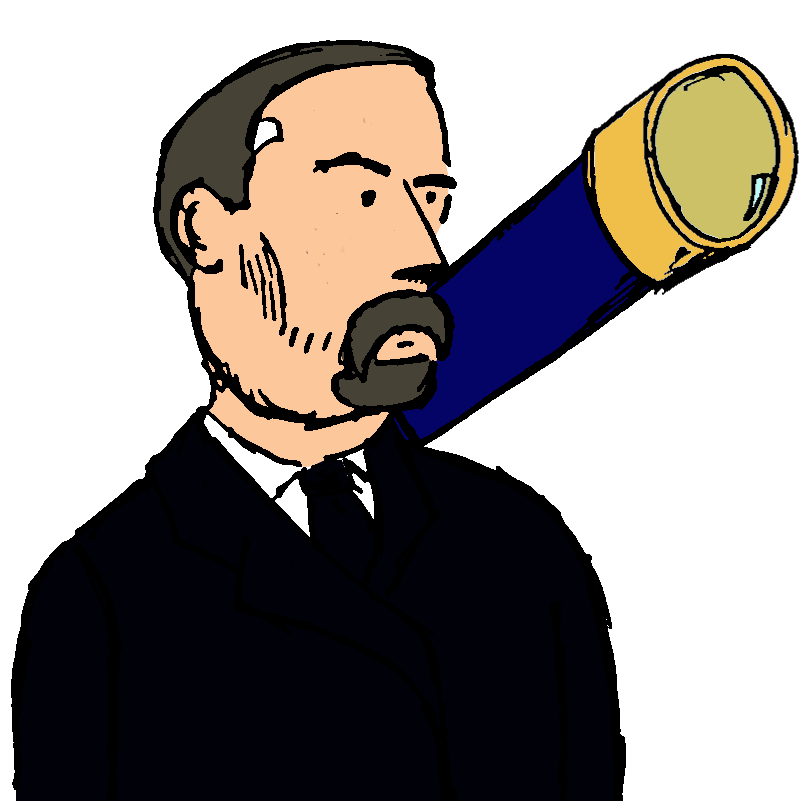
\includegraphics[width=10cm]{schiaparelli}};
			%
			\node at (21,3) {\textcolor{black}{\fontsize{23}{24}\selectfont Giovanni Schiaparelli, direttore}};
			\node at (21,2) {\textcolor{black}{\fontsize{23}{24}\selectfont dell'Osservatorio Astronomico di}};
			\node at (21,1) {\textcolor{black}{\fontsize{23}{24}\selectfont Brera, famoso per le sue}};
			\node at (21,0) {\textcolor{black}{\fontsize{23}{24}\selectfont osservazioni sul pianeta Marte,}};
			\node at (21,-1) {\textcolor{black}{\fontsize{23}{24}\selectfont nel 1889 aveva comunicato che, dai}};
			\node at (21,-2) {\textcolor{black}{\fontsize{23}{24}\selectfont suoi calcoli, Mercurio esponeva al}};
			\node at (21,-3) {\textcolor{black}{\fontsize{23}{24}\selectfont Sole sempre la stessa faccia.}};
			%
			\draw [fill=dida, ultra thick] (1,-8) rectangle (18,-16);
			%
			\draw[fill=red!50!mercury, ultra thick] (23,-12) circle (5cm);
			\draw (25,-12) [fill=mercury, partial ellipse=101:259:5 and 5] (23,-12) [fill=mercury, partial ellipse=78:-78:5 and 5];
			\draw (28,-12) [fill=earth, opacity=0.4, partial ellipse=120:240:5 and 5] (23,-12) [fill=earth, opacity=0.4, partial ellipse=60:-60:5 and 5];
			%
			\node at (9.5,-9) {\textcolor{black}{\fontsize{23}{24}\selectfont Da qui le teorie sulla superficie}};
			\node at (9.5,-10) {\textcolor{black}{\fontsize{23}{24}\selectfont mercuriana supponevano che il "lato}};
			\node at (9.5,-11) {\textcolor{black}{\fontsize{23}{24}\selectfont illuminato" presentasse metallo fuso,}};
			\node at (9.5,-12) {\textcolor{black}{\fontsize{23}{24}\selectfont mentre il "lato oscuro" presentasse}};
			\node at (9.5,-13) {\textcolor{black}{\fontsize{23}{24}\selectfont l'atmosfera primordiale in forma}};
			\node at (9.5,-14) {\textcolor{black}{\fontsize{23}{24}\selectfont ghiacciata. I due lati erano separati}};
			\node at (9.5,-15) {\textcolor{black}{\fontsize{23}{24}\selectfont da una "zona crepuscolare".}};
			%
			\draw[fill=space, ultra thick] (1,-17.5) rectangle (29,-30.5);
			\draw[ultra thick, color=white] (7,-30) -- (7,-29);
			\draw[fill=mercury, ultra thick] (7,-24) circle (5cm);
			\draw[->,ultra thick, color=white] (7,-20) -- (7,-18);
			\draw (7,-24) [->,ultra thick, color=white, partial ellipse=200:340:6 and 3];
			%
			\node at (21,-19) {\textcolor{white}{\fontsize{23}{24}\selectfont Nel 1965 le osservazioni condotte}};
			\node at (21,-20) {\textcolor{white}{\fontsize{23}{24}\selectfont da Gordon Pettengill e R. Dyce}};
			\node at (21,-21) {\textcolor{white}{\fontsize{23}{24}\selectfont indicarono che Mercurio compiva}};
			\node at (21,-22) {\textcolor{white}{\fontsize{23}{24}\selectfont una rotazione intorno al suo asse}};
			\node at (21,-23) {\textcolor{white}{\fontsize{23}{24}\selectfont in circa 59 giorni. Questo permise}};
			\node at (21,-24) {\textcolor{white}{\fontsize{23}{24}\selectfont a Giuseppe Colombo di concludere}};
			\node at (21,-25) {\textcolor{white}{\fontsize{23}{24}\selectfont che il suo periodo di rotazione era}};
			\node at (21,-26) {\textcolor{white}{\fontsize{23}{24}\selectfont circa due terzi di quello orbitale.}};
			\node at (21,-27) {\textcolor{white}{\fontsize{23}{24}\selectfont Dunque la rotazione di Mercurio non}};
			\node at (21,-28) {\textcolor{white}{\fontsize{23}{24}\selectfont è sincrona come aveva suggerito}};
			\node at (21,-29) {\textcolor{white}{\fontsize{23}{24}\selectfont Schiaparelli intorno al 1880.}};
		\end{scope}
		%orbit
		\begin{scope}[shift={(0,-108)}]
			\draw [fill=space, ultra thick] (2,17) rectangle (20,-5);
			\draw [fill=white] (11,0) circle (2cm);
			%
			\foreach \i in {-1,0,1}
			{\begin{scope}[rotate around={(\i * 15):(11,0)}]
				\draw [color=white, ultra thick] (11,6) ellipse (6cm and 10cm);
				\draw [fill=mercury] (11,16) circle (0.5cm);
			\end{scope}}
			%
			\draw [fill=dida, thick] (20,14) rectangle (30,-2);
			\node at (25,13) {\textcolor{black}{\fontsize{23}{24}\selectfont L'orbita di Mercurio}};
			\node at (25,12) {\textcolor{black}{\fontsize{23}{24}\selectfont risulta ellittica solo}};
			\node at (25,11) {\textcolor{black}{\fontsize{23}{24}\selectfont in prima}};
			\node at (25,10) {\textcolor{black}{\fontsize{23}{24}\selectfont approssimazione.}};
			\node at (25,9) {\textcolor{black}{\fontsize{23}{24}\selectfont Questo a causa della}};
			\node at (25,8) {\textcolor{black}{\fontsize{23}{24}\selectfont precessione del}};
			\node at (25,7) {\textcolor{black}{\fontsize{23}{24}\selectfont perielio, il punto di}};
			\node at (25,6) {\textcolor{black}{\fontsize{23}{24}\selectfont minima distanza dal}};
			\node at (25,5) {\textcolor{black}{\fontsize{23}{24}\selectfont Sole.}};
			\node at (25,4) {\textcolor{black}{\fontsize{23}{24}\selectfont Tale anomalia venne}};
			\node at (25,3) {\textcolor{black}{\fontsize{23}{24}\selectfont spiegata per la prima}};
			\node at (25,2) {\textcolor{black}{\fontsize{23}{24}\selectfont volta nel 1915 da}};
			\node at (25,1) {\textcolor{black}{\fontsize{23}{24}\selectfont Albert Einstein grazie}};
			\node at (25,0) {\textcolor{black}{\fontsize{23}{24}\selectfont alla teoria della}};
			\node at (25,-1) {\textcolor{black}{\fontsize{23}{24}\selectfont relatività generale.}};
		\end{scope}
		%structure
		\begin{scope}[shift={(0,-126)}]
			\draw [fill=earth, opacity=0.4] (15,0) circle (11cm);
			\draw [fill=mercury,ultra thick] (15,0) circle (10cm);
			\draw [fill=craterm] (15,0) [partial ellipse=-90:90:9.5 and 9.5] (15,0) [partial ellipse=90:270:4 and 9.5];
			%
			\draw [fill=core2] (15,0) [partial ellipse=-90:90:8.8 and 8.8] (15,0) [partial ellipse=90:270:3.4 and 8.8];
			\draw (15,9.5) -- (15,-9.5);
			\draw [fill=core1] (15,0) [partial ellipse=-90:90:7.3 and 7.3] (15,0) [partial ellipse=90:270:2.5 and 7.3];
			%
			\draw [<-,ultra thick] (16,9) -- (20.3,10);
			\draw [fill=dida,thick] (20.3,10) rectangle (27.2,12);
			\node at (22,11.5) {\textcolor{black}{\fontsize{23}{24}\selectfont crosta}};
			\node at (23.8,10.5) {\textcolor{black}{\fontsize{15}{16}\selectfont spessore: 100-200 km}};
			%
			\draw [<-,ultra thick] (16,7.9) -- (21.8,8.2);
			\draw [fill=dida,thick] (21.8,7.7) rectangle (27.4,9.7);
			\node at (24,9.2) {\textcolor{black}{\fontsize{23}{24}\selectfont mantello}};
			\node at (24.6,8.2) {\textcolor{black}{\fontsize{15}{16}\selectfont spessore: 600 km}};
			%
			\draw [<-,ultra thick] (16,2.3) -- (22.3,5.4);
			\draw [fill=dida,thick] (22.3,5.4) rectangle (27.5,7.4);
			\node at (24,6.9) {\textcolor{black}{\fontsize{23}{24}\selectfont nucleo}};
			\node at (24.9,5.9) {\textcolor{black}{\fontsize{15}{16}\selectfont raggio: 1800 km}};
			%
			\draw [->,ultra thick] (13,-12) -- (15,-10.5);
			\draw [fill=dida,thick] (2.8,-12) rectangle (22.2,-17);
			\node at (12.2,-13) {\textcolor{black}{\fontsize{23}{24}\selectfont Mercurio non possiede una vera e propria}};
			\node at (12,-14) {\textcolor{black}{\fontsize{23}{24}\selectfont atmosfera, ma si possono trovare tracce}};
			\node at (12.2,-15) {\textcolor{black}{\fontsize{23}{24}\selectfont di alcuni gas: ossigeno ($42 \, \%$), sodio ($29 \, \%$),}};
			\node at (12.5,-16) {\textcolor{black}{\fontsize{23}{24}\selectfont idrogeno ($22 \, \%$), elio ($6 \, \%$) e potassio ($0.5 \, \%$).}};
		\end{scope}
		%
		\begin{scope}[shift={(0,-144.5)}]
			\node at (27,0) () {
\includegraphics[width=3.7cm]{licenza}};
			\node at (18,-0.1) {\textcolor{black}{\fontsize{14}{15}\selectfont Testo e illustrazioni: @ulaulaman - Gianluigi Filippelli}};
		\end{scope}
	\end{tikzpicture}
%
\end{document}
